\mysection{Objectif}
L'objectif de ce document est faire un rapport du stage, qui détaille le lieu de travail, les productions du stage en expliquant les méthodes utilisées et qui montre les résultats obtenus, les commente et présente les implications des conclusions.
\mysection{Introduction Générale}
Afin de compléter la formation du 2A CentraleSupélec, un stage a été réalisé entre les mois de juillet et septembre de 2017, au sein de l'équipe \gls{AUT} du	
\gls{IETR} en travaillant au cadre du projet d'\title, avec l'orientation de M. Hervé GUÉGUEN.


\mysubsection{Sur le lieu de travail} 
\mysubsubsection{L'IETR}
L'IETR est un institut de recherche français, spécialisé en électronique et télécommunication, localisé à Rennes, regroupant plus de 300 enseignants-chercheurs, ingénieurs, doctorants et administratifs, issus des écoles et instituts de recherche de la région comme le CNRS, l'Université Rennes 1, INSA de Rennes, CentraleSupélec et Université de Nantes.

L'IETR a une liste considérable de partenaires, incluant des centres publics comme le CEA, le CNES et le Club Automatique et Automatisation industrielle de la SEE, des petites et moyennes entreprises privés comme A\&P Lithos, Adlightec et Advansee, et des grandes groupes comme Alstom, EDF et Mitsubishi. 

Son partenariat International compte sur plus de 70 Universités, Instituts et Agences de recherche parmi tout le monde, incluent \gls{JPL}, \gls{Polimi} et \gls{USP}.

\mysubsubsection{Division des Équipes de Recherche}
Afin de meilleur catégoriser les thématiques des projets de recherche L'IETR est divisé en 6 départements/équipes:

\begin{itemize}
	\item Antennes \& Dispositifs Hyperfréquences (ADH)
	\item Signal \& Communications (SC)
	\item Ondes \& Signaux (OS)
	\item Image
	\item Microélectronique \& Microcapteurs (MM)
	\item Automatique (AUT)
\end{itemize}

L'organigramme structurel intégrant tant les parties de recherche que les parties administratives du IETR peut être vu dans la figure \ref{fig:organigramme_IETR_160717_v28}.
\pagebreak

\mysubsubsection{L'équipe AUT}
L'équipe de Automatique est basée a CentraleSupélec et travaille dans diverses thématiques utilisant les connaissances des domaines d'analyse et commande des systèmes hybrides.

Ses projets ont des applications qui couvrent diverses métiers, on peut voir quelques exemples de projets: comme dans le métier des bâtiments intelligents ( régulation de chauffage pour augmenter l'efficience énergétique )  ,  de la santé ( models des pancréas artificiels pour contrôler le métabolisme de glucose ), du transport ( stratégies de régulation de vitesse des automobiles) , de la distribution d'énergie ( Études de stabilisation en tension de générateurs distribués dans un réseau de distribution ) entre autres.

\vspace{.5cm}
\begin{figure}[H]
	\begin{center}	
		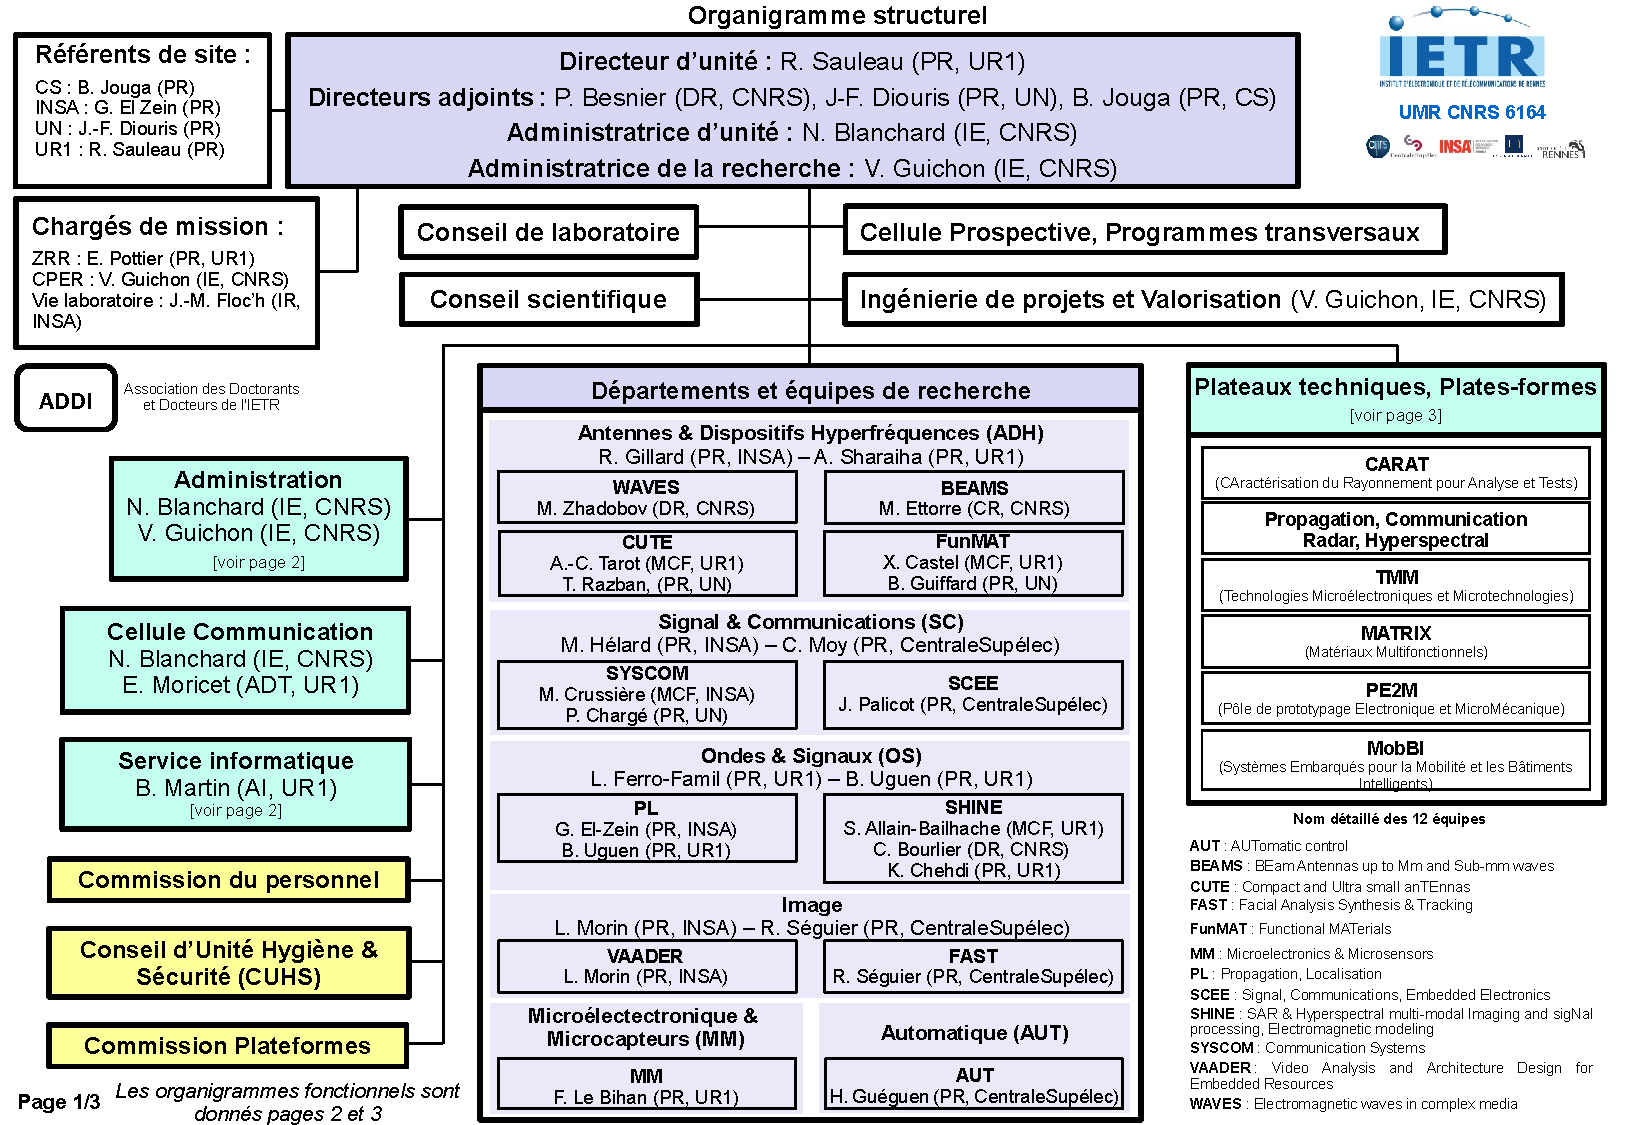
\includegraphics[width=\textwidth]{./organigramme_IETR_160717_v28.pdf}
		\caption{Organigramme du IETR.}
		\label{fig:organigramme_IETR_160717_v28}
	\end{center}
\end{figure}












